\documentclass[11pt]{article}
\usepackage[margin=1in]{geometry}
\usepackage{amsmath,amssymb,booktabs,graphicx,setspace,caption,hyperref}
\usepackage[T1]{fontenc}
\usepackage{mathpazo}
\setlength{\parindent}{0pt}
\setlength{\parskip}{0.6em}
\captionsetup{font=small,skip=6pt}
\title{Panel MS-AR(1) with random-effects intercepts, 1970Q1 onward\\[0.4em]\large Pulled real GDP per worker}
\author{}
\date{}
\begin{document}
\maketitle
\section{Model}
Joint panel Markov-switching AR(1) around a \emph{linear} trend, with three regimes:
\begin{align}
y_{it} &= a_i + g\, t + z_{it}, \\
z_{i,t+1} &= \bigl(1-\rho(s_{it})\bigr)\mu(s_{it}) + \rho(s_{it})\, z_{it} + \sigma(s_{it})\,\varepsilon_{it}, \\
s_{i,t+1} &\sim \Pi(\,\cdot\mid s_{it}), \\
a_i &\sim \mathcal{N}(\alpha,\omega^2) \quad \text{(random effects)}.
\end{align}
The outcome is log real GDP per worker from the pulled quarterly panel (constant 2015 USD, market FX). The trend is linear in calendar time $t$ ($g$ per year, common across countries). In the pooled specification $a_i\equiv a$. In the random-effects specification the $a_i$ are i.i.d.\ Normal draws; $\alpha$ and $\omega$ are estimated by maximum likelihood, integrating each country's Hamilton-filter likelihood by 11-point Gauss--Hermite quadrature. Cycles are plotted using the posterior mean of $a_i$. Latent paths $s_{it}$ are country-specific. The regime dated $t$ governs the transition from $z_t$ to $z_{t+1}$. $\sigma$ and $\rho$ switch with the regime. The median $\mu$ is pinned at 0. $|\rho|<0.995$.
Standard errors (in parentheses) are delta-method from a numerical Hessian on shared parameters. $\pi$ is the ergodic distribution of $\Pi$. $E[z]$ is the long-run mean of the cycle implied by $\mu$, $\rho$, and $\Pi$.
\clearpage
\section{Common intercept and linear trend}
Pulled panel from 1970Q1: log real GDP per worker. 101 countries, 7354 observations, 1970-Q1--2026-Q2. Fitted countries: 92. Observations: 6787. Log-likelihood: 14863.42. Ergodic mean of the cycle $E[z]=-0.0985$ (0.1273).
Common intercept $a=10.4145$ (0.1330). Common slope $g=0.0037$ (0.0010).
\begin{table}[h]
\centering
\caption{Regime AR(1), transition matrix, and ergodic $\pi$. Columns are regimes.}
\begin{tabular}{lccc}
\toprule
 & (0) & (1) & (2) \\
\midrule
$\mu$ & -1.2653 & 0.0000 & 0.8509 \\
 & (0.1601) & --- & (0.0994) \\ \addlinespace
$\sigma$ & 0.1217 & 0.0272 & 0.0111 \\
 & (0.0032) & (0.0006) & (0.0002) \\ \addlinespace
$\rho$ & 0.9905 & 0.9950 & 0.9950 \\
 & (0.0020) & (0.0000) & (0.0000) \\ \addlinespace
$\Pi_{0\cdot}$ & 0.9328 & 0.0570 & 0.0102 \\
 & (0.0095) & (0.0092) & (0.0042) \\ \addlinespace
$\Pi_{1\cdot}$ & 0.0175 & 0.9591 & 0.0234 \\
 & (0.0034) & (0.0048) & (0.0041) \\ \addlinespace
$\Pi_{2\cdot}$ & 0.0147 & 0.0157 & 0.9697 \\
 & (0.0032) & (0.0040) & (0.0037) \\ \addlinespace
$\pi$ & 0.1937 & 0.4187 & 0.3876 \\
 & (0.0227) & (0.0305) & (0.0330) \\ \addlinespace
\bottomrule
\end{tabular}
\end{table}
\begin{figure}[h]
\centering
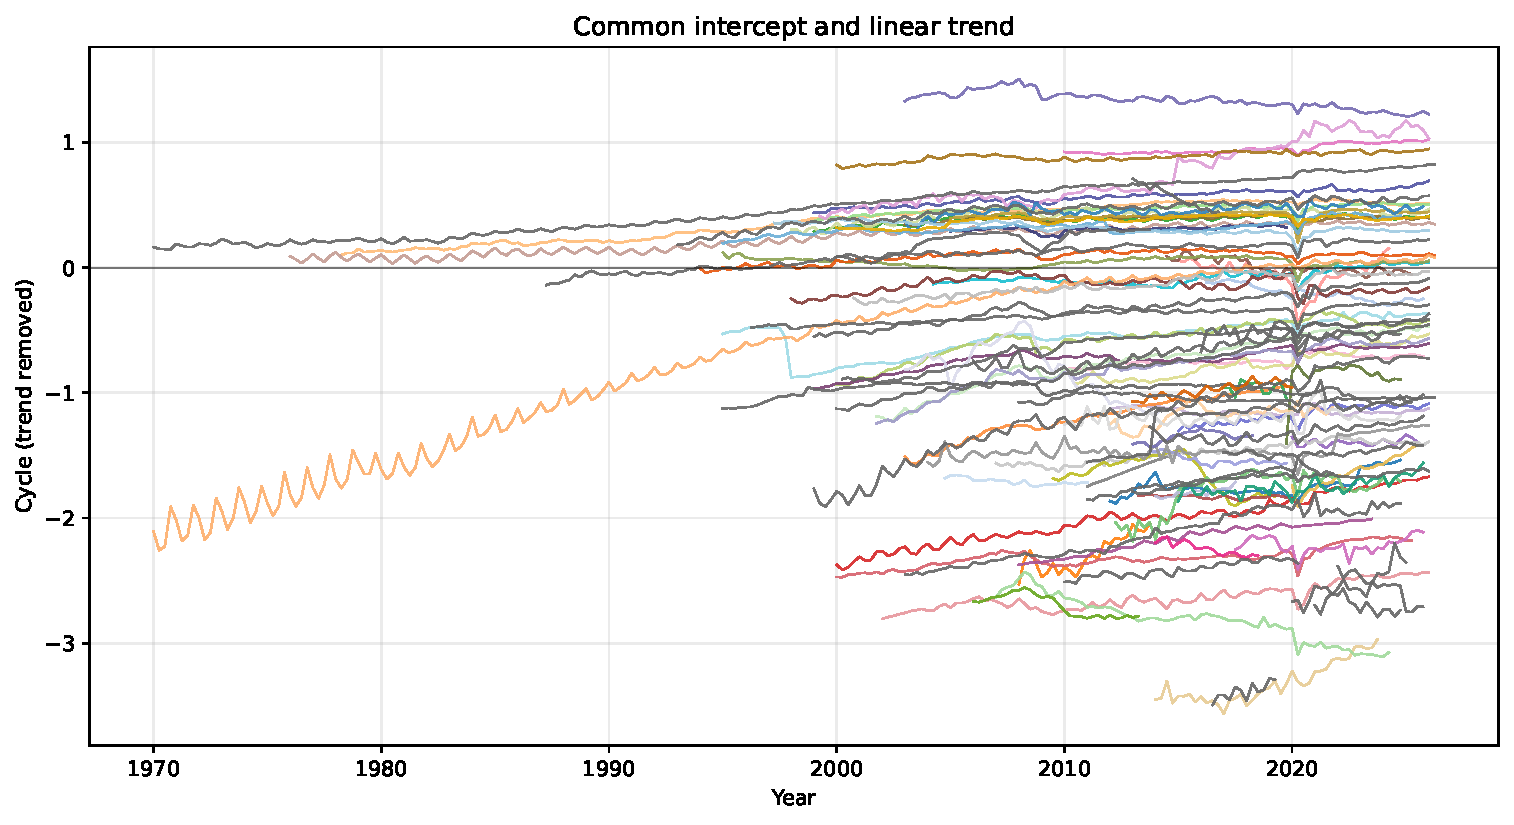
\includegraphics[width=0.75\textwidth]{figs/cycle_pulled_common_ag.pdf}
\caption{Country cycles after removing the linear trend.}
\end{figure}
\clearpage
\section{Random-effects intercepts, common linear trend}
Pulled panel from 1970Q1: log real GDP per worker. 101 countries, 7354 observations, 1970-Q1--2026-Q2. Fitted countries: 92. Observations: 6787. Log-likelihood: 15090.50. Ergodic mean of the cycle $E[z]=-0.1636$ (0.1083).
Random intercepts $a_i\sim N(\alpha,\omega^2)$ with $\alpha=9.8429$ (0.0823), $\omega=0.7204$ (0.0238). Posterior-mean $a_i$: mean 9.845, min 7.996, max 11.684. Common slope $g=0.0084$ (0.0008).
\begin{table}[h]
\centering
\caption{Regime AR(1), transition matrix, and ergodic $\pi$. Columns are regimes.}
\begin{tabular}{lccc}
\toprule
 & (0) & (1) & (2) \\
\midrule
$\mu$ & -0.8152 & 0.0000 & 0.5277 \\
 & (0.1955) & --- & (0.0827) \\ \addlinespace
$\sigma$ & 0.1244 & 0.0271 & 0.0109 \\
 & (0.0032) & (0.0006) & (0.0002) \\ \addlinespace
$\rho$ & 0.9804 & 0.9950 & 0.9950 \\
 & (0.0081) & (0.0002) & (0.0000) \\ \addlinespace
$\Pi_{0\cdot}$ & 0.9351 & 0.0490 & 0.0159 \\
 & (0.0096) & (0.0089) & (0.0051) \\ \addlinespace
$\Pi_{1\cdot}$ & 0.0123 & 0.9700 & 0.0177 \\
 & (0.0027) & (0.0041) & (0.0033) \\ \addlinespace
$\Pi_{2\cdot}$ & 0.0125 & 0.0126 & 0.9749 \\
 & (0.0028) & (0.0033) & (0.0033) \\ \addlinespace
$\pi$ & 0.1605 & 0.4323 & 0.4071 \\
 & (0.0209) & (0.0329) & (0.0339) \\ \addlinespace
\bottomrule
\end{tabular}
\end{table}
\begin{figure}[h]
\centering
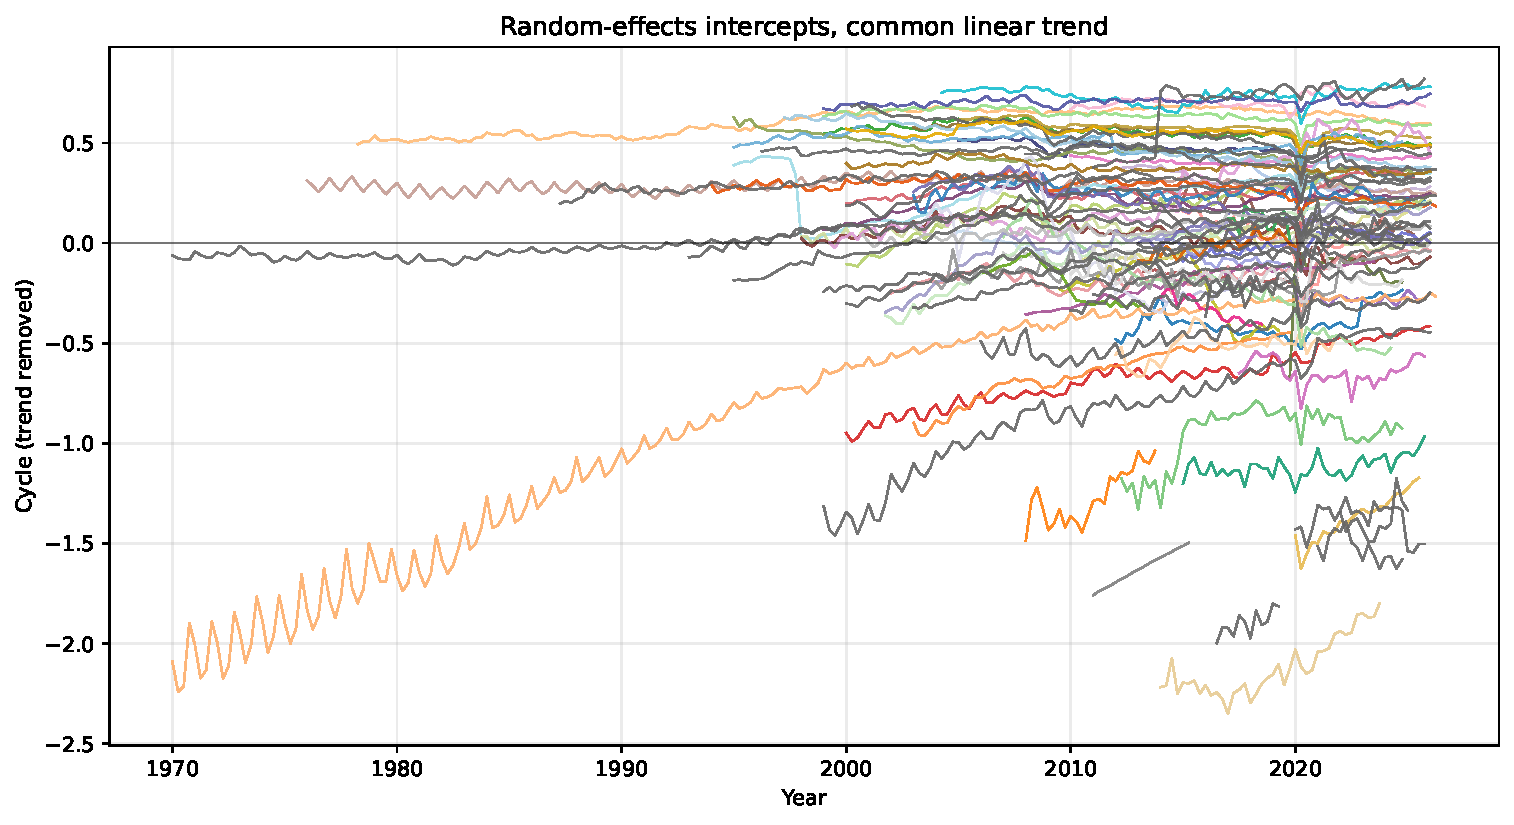
\includegraphics[width=0.75\textwidth]{figs/cycle_pulled_re_ai.pdf}
\caption{Country cycles after removing the linear trend.}
\end{figure}
\end{document}
